% =============================================================================
% MASTER'S THESIS PROPOSAL — MIT Program, Tribhuvan University
% Title: Enhancing Self-Supervised Video Representations with HAF-STD Net: A Comparative Evaluation Against VLM for Action Recognition
% =============================================================================

\documentclass[a4paper, 12pt]{report}

% --- Packages ----------------------------------------------------------------
\usepackage[top=1in, bottom=1in, left=1.5in, right=1in]{geometry}
\usepackage{times}                    % Times New Roman
\usepackage{setspace}                 % 1.5 spacing
\usepackage{graphicx}
\usepackage{amsmath, amssymb}
\usepackage{booktabs}
\usepackage{longtable}
\usepackage{multirow}
\usepackage{array}
\usepackage{tabularx}
\usepackage{float}
\usepackage{caption}
\usepackage{subcaption}
\usepackage[hidelinks]{hyperref}
\usepackage{url}
\usepackage[style=apa, backend=biber, natbib=true]{biblatex}
\addbibresource{references.bib}
\usepackage{algorithm}

\usepackage{algorithmic}
\usepackage{listings}
\usepackage{xcolor}
\usepackage{tikz}
\usepackage{pgfplots}
\pgfplotsset{compat=1.18}
\usepackage{pgfgantt}
\usepackage{enumitem}
\usepackage{fancyhdr}
\usepackage{tocloft}
\usepackage{titlesec}

% --- Spacing -----------------------------------------------------------------
\onehalfspacing

% --- Heading Sizes (as per TU IoST Regulation) ------------------------------
\titleformat{\chapter}[display]
  {\normalfont\fontsize{16}{19}\bfseries}
  {\chaptertitlename\ \thechapter}{12pt}{\fontsize{16}{19}\bfseries}
\titleformat{\section}
  {\normalfont\fontsize{14}{17}\bfseries}{\thesection}{1em}{}
\titleformat{\subsection}
  {\normalfont\fontsize{12}{14}\bfseries}{\thesubsection}{1em}{}
\titleformat{\subsubsection}
  {\normalfont\fontsize{12}{14}\bfseries}{\thesubsubsection}{1em}{}

% --- Page style --------------------------------------------------------------
\pagestyle{fancy}
\fancyhf{}
\fancyfoot[C]{\thepage}
\renewcommand{\headrulewidth}{0pt}

% --- Caption style -----------------------------------------------------------
\captionsetup{font={bf,normalsize}, labelsep=colon}

% --- Author variables --------------------------------------------------------
\newcommand{\authorname}{Erize Rai}
\newcommand{\studentroll}{8025006}
\newcommand{\turegdno}{5-3-28-193-2023}
\newcommand{\thesistitle}{Enhancing Self-Supervised Video Representations with HAF-STD Net: A Comparative Evaluation Against VLM for Action Recognition}

% --- Custom commands ---------------------------------------------------------
\newcommand{\vjepaa}{V-JEPA~2.1}
\newcommand{\qwenvl}{Qwen2.5-VL}
% --- biblatex-apa provides \citep, \citet natively via natbib=true ---


% =============================================================================
\begin{document}

% Roman numerals for front matter
\pagenumbering{roman}

% --- Front Matter ------------------------------------------------------------
% =============================================================================
%        TITLE PAGE — TU IoST Thesis Proposal Format
%        (Matches reference image layout exactly)
% =============================================================================

\begin{titlepage}
\centering

\vspace*{0.2cm}

{\fontsize{18}{22}\selectfont \textbf{Enhancing Self-Supervised Video Representations with HAF-STD Net: A Comparative Evaluation Against VLM for Action Recognition}}\\[1.5cm]

% --- TU Logo (centered) -----------------------------------------------------

\includegraphics[width=2in]{../fig/tulogo.png}\\[2.0cm]

% --- Submission statement ----------------------------------------------------
{\fontsize{14}{18}\selectfont \textbf{A Thesis Proposal Submitted to the}}\\[0.15cm]
{\fontsize{14}{18}\selectfont \textbf{Central Department of Computer Science and Information Technology}}\\[0.15cm]
{\fontsize{14}{18}\selectfont \textbf{Tribhuvan University, Kirtipur, Kathmandu, Nepal}}\\[0.15cm]
{\fontsize{14}{18}\selectfont \textbf{for Approval}}\\[1.5cm]

% --- By ----------------------------------------------------------------------
{\fontsize{14}{18}\selectfont By}\\[0.6cm]

% --- Student details ---------------------------------------------------------
{\fontsize{14}{18}\selectfont \textbf{\authorname}}\\[0.1cm]
{\fontsize{14}{18}\selectfont \textbf{Symbol No.: \studentroll}}\\[0.1cm]
{\fontsize{14}{18}\selectfont \textbf{T.U. Registration No.: \turegdno}}\\[1.5cm]

% --- Month, Year -------------------------------------------------------------
{\fontsize{14}{18}\selectfont \textbf{NOVEMBER, 2026}}

\end{titlepage}

% % =============================================================================
%                   DECLARATION FROM THE STUDENT (PROPOSAL)
% =============================================================================

\clearpage
\phantomsection
\addcontentsline{toc}{chapter}{Declaration}

\begin{center}
{\fontsize{16}{20}\selectfont \textbf{Declaration}}
\end{center}

\vspace{0.5cm}

\noindent
I hereby declare that the thesis proposal entitled \textbf{``\thesistitle''} submitted to the Central Department of Computer Science and Information Technology, Institute of Science and Technology (IoST), Tribhuvan University, Nepal is an original work prepared under the supervision of \textbf{}. This proposal has not been submitted earlier in part or full to any other institution for the award of any degree.

\vspace{3cm}

\noindent
\begin{tabular}{@{}l}
\rule{6cm}{0.4pt} \\
\textbf{\authorname} \\
Symbol No.: \studentroll \\
T.U. Regd. No.: \turegdno \\
\end{tabular}

\vspace{1cm}
\noindent
Date: NOVEMBER, 2026
  % Removed
% % =============================================================================
%              RECOMMENDATION FROM THE SUPERVISOR (PROPOSAL)
% =============================================================================

\clearpage
\phantomsection
\addcontentsline{toc}{chapter}{Recommendation}

\begin{center}
{\fontsize{16}{20}\selectfont \textbf{Recommendation}}
\end{center}

\vspace{0.5cm}

\noindent
This is to recommend that \textbf{\authorname} (Symbol No.: \studentroll, T.U. Registration No.: \turegdno) has prepared this thesis proposal entitled \textbf{``\thesistitle''} under my supervision. To my knowledge, this work is original and has not been submitted to any other institution for the award of any degree. I recommend this proposal for approval.

\vspace{2.5cm}

\noindent
\begin{tabular}{@{}p{7.5cm}p{7.5cm}@{}}
\rule{6cm}{0.4pt} & \rule{6cm}{0.4pt} \\
\textbf{Supervisor} & \textbf{Co-Supervisor} \\
Asst. Prof. Dr. Dhiraj Kedar Pandey &  \\
Assistant Professor &  \\
Central Department of Computer Science & Central Department of Computer Science \\
and Information Technology & and Information Technology \\
Tribhuvan University & Tribhuvan University, Kathmandu, Nepal \\
Kathmandu, Nepal & \\
\end{tabular}

\vspace{1.5cm}

\begin{center}
{\fontsize{12}{15}\selectfont \textbf{NOVEMBER, 2026}}
\end{center}
  % Removed

% --- Table of Contents -------------------------------------------------------
\clearpage
\phantomsection
\addcontentsline{toc}{chapter}{Table of Contents}
\tableofcontents

% --- Lists -------------------------------------------------------------------
\clearpage
\phantomsection
\addcontentsline{toc}{chapter}{List of Figures}
\listoffigures

\clearpage
\phantomsection
\addcontentsline{toc}{chapter}{List of Tables}
\listoftables

\clearpage
% =============================================================================
%                  LIST OF ABBREVIATIONS
% =============================================================================
\chapter*{List of Abbreviations}
\addcontentsline{toc}{chapter}{List of Abbreviations}

\begin{longtable}{@{}p{3.5cm}p{10cm}@{}}
\toprule
\textbf{Abbreviation} & \textbf{Full Form} \\
\midrule
\endhead
AI & Artificial Intelligence \\
BB & Balance Beam \\
CNN & Convolutional Neural Network \\
FX & Floor Exercise \\
GPU & Graphics Processing Unit \\
HMDB & Human Motion DataBase \\
JEPA & Joint Embedding Predictive Architecture \\
MAE & Masked Autoencoder \\
MCC & Matthews Correlation Coefficient \\
MIT & Master of Information Technology \\
MLP & Multi-Layer Perceptron \\
NF4 & Normal Float 4-bit (Quantization Format) \\
PCA & Principal Component Analysis \\
RBF & Radial Basis Function \\
SDPA & Scaled Dot-Product Attention \\
SSL & Self-Supervised Learning \\
SVM & Support Vector Machine \\
UB & Uneven Bars \\
V-JEPA & Video Joint Embedding Predictive Architecture \\
ViT & Vision Transformer \\
VLM & Vision-Language Model \\
VT & Vault \\
\bottomrule
\end{longtable}


% =============================================================================
%      MAIN REPORT — Arabic numerals from here
% =============================================================================
\clearpage
\pagenumbering{arabic}
\setcounter{page}{1}

% --- Chapters ----------------------------------------------------------------
% =============================================================================
%               CHAPTER 1: INTRODUCTION
% =============================================================================
\chapter{Introduction}

\section{Introduction}

Video understanding represents one of the most challenging frontiers in computer vision and artificial intelligence research. Unlike static image recognition, which has seen remarkable progress over the past decade, video comprehension demands that models capture not only spatial features within individual frames but also the complex temporal dynamics that unfold across sequences of frames \citep{bardes2024vjepa}. This temporal dimension introduces an exponential increase in computational complexity and representational challenges, making video understanding a substantially more demanding task than its image-based counterpart.

Action recognition---the task of identifying human activities from video data---is a central problem in video understanding with broad applications spanning sports analytics, surveillance, human-computer interaction, healthcare monitoring, and content-based video retrieval \citep{bordes2024vlm}. The difficulty of action recognition varies dramatically depending on the granularity of the target classes: coarse-grained recognition of clearly distinct activities (e.g., ``running'' vs.\ ``swimming'') differs fundamentally from fine-grained recognition of visually similar activities (e.g., distinguishing between gymnastics events that occur in similar arenas).

Two fundamentally different paradigms have emerged for learning video representations in recent years. Self-Supervised Learning (SSL) enables models to learn representational features from unlabeled video data by solving predictive latent pretext tasks, such as predicting masked spatiotemporal regions without pixel reconstruction \citep{assran2023ijepa, assran2025vjepa2}. Vision-Language Modeling (VLM), on the other hand, pre-trains models on massive multimodal paired visual and textual datasets using visual instruction tuning and autoregressive language modeling objectives \citep{bordes2024vlm, qwen2025qwen3vl}.

Both paradigms have produced models that achieve impressive state-of-the-art results on standard benchmarks, yet their relative representational capabilities across different levels of recognition granularity remain insufficiently explored. This research proposes a systematic comparative analysis between a leading model from each paradigm: \vjepaa{} \citep{assran2025vjepa2}, a self-supervised video encoder developed by Meta AI with 654 million parameters, and \qwenvl{} \citep{qwen2025qwen3vl}, an instruction-tuned vision-language model with 7 billion parameters. The evaluation is conducted on two benchmark datasets: FineGym (fine-grained gymnastics event classification) and HMDB51 (coarse-grained human action recognition).

\section{Problem Statement}

Despite recent advancements in video foundation models, several critical research gaps persist in the literature. Existing studies evaluate self-supervised video encoders and vision-language models in isolation, using disparate datasets, evaluation protocols, and fine-tuning setups, and direct controlled comparisons of their representation quality under identical frozen-feature evaluation protocols are missing. Furthermore, while both paradigms excel on specific benchmarks, how their relative performance changes across different levels of task granularity---from fine-grained domain-specific actions (FineGym, 4 classes) to coarse-grained general actions (HMDB51, 51 classes)---has not been systematically investigated. \vjepaa{} (654M parameters) is approximately $10\times$ smaller than \qwenvl{} (7B parameters), and it remains an open question whether massive parameter scale in general-purpose VLMs translates to superior video action representations compared to compact, video-specialized self-supervised encoders.

The problem is therefore not only whether frozen self-supervised latent prediction encoders can learn more discriminative temporal representations than large vision-language models, but whether compact, video-specialized architectures can match or exceed the representational quality of models with an order-of-magnitude more parameters across varying task granularities.

\section{Objectives}

The objectives of this study are:
\begin{enumerate}[leftmargin=*]
    \item To evaluate and compare the effectiveness of self-supervised video representations (\vjepaa{}) and vision-language representations (\qwenvl{}) for video action recognition across fine-grained (FineGym) and coarse-grained (HMDB51) task granularities.
    \item To design, implement, and evaluate a specialized classification architecture HAF-STD Net (Hierarchical Adaptive Fusion with Spectral-Temporal Decomposition) tailored for frozen self-supervised video representations.
\end{enumerate}


% =============================================================================
%    CHAPTER 2: BACKGROUND STUDY AND LITERATURE REVIEW
% =============================================================================
\chapter{Background Study and Literature Review}

\section{Background Study}

Traditional self-supervised learning approaches in computer vision have relied either on generative pixel reconstruction or on contrastive learning across augmented views. Pixel reconstruction forces models to spend representational capacity on high-frequency, unessential visual details, while contrastive learning requires large batch sizes and carefully designed negative sampling. To address these limitations, Joint Embedding Predictive Architectures (JEPA) perform non-generative prediction directly within a learned latent feature space. \citet{assran2023ijepa} introduced Image-JEPA (I-JEPA), demonstrating that predicting missing target representations from context patches in latent space produces highly semantically rich visual embeddings.

Extending the JEPA paradigm to temporal data, \citet{bardes2024vjepa} proposed V-JEPA, which applies feature prediction to spatiotemporal video blocks. Subsequently, \citet{assran2025vjepa2} developed \vjepaa{}, scaling video latent prediction using a ViT-Huge backbone (654M parameters) trained on extensive unlabelled video collections. Most recently, \citet{murlabadia2026vjepa21} introduced V-JEPA 2.1, incorporating a dense predictive loss and multi-layer intermediate supervision to enhance spatial and temporal feature grounding. Variational extensions to JEPA have also been explored by \citet{huang2026vjepa}, who proposed Variational JEPA (VJEPA), introducing a probabilistic latent prediction framework that models distribution uncertainty for stochastic control and predictive world modeling.

Parallel to self-supervised feature learning, Vision-Language Models (VLMs) have emerged as powerful general-purpose foundation models. As surveyed by \citet{bordes2024vlm} and \citet{zhang2023vlmsurvey}, VLMs connect visual encoders with autoregressive language model decoders through visual instruction tuning. Recent developments in vision-language architectures include the \qwenvl{} technical report \citep{bai2025qwen2vl} and Qwen3-VL \citep{qwen2025qwen3vl}, which support native spatiotemporal visual tokenization, variable frame resolution, and long-context multimodal understanding. To enable practical deployment under strict hardware resource boundaries, \citet{pathak2026efficientvlms} reviewed quantization, pruning, and low-bit inference techniques for large vision-language models.

\section{Literature Review}


The progression from Image-JEPA to V-JEPA~2.1 reveals a systematic trajectory of architectural refinement aimed at producing increasingly expressive latent representations. \citet{assran2023ijepa} first established the foundational principle that predicting target patch representations from context patches---without pixel-level reconstruction---produces semantically richer embeddings than generative or contrastive alternatives. Their Image-JEPA demonstrated that a non-generative latent predictive objective avoids wasting model capacity on perceptually irrelevant high-frequency detail, while simultaneously eliminating the dependency on hand-crafted data augmentations inherent to contrastive learning pipelines.

Building on this image-level foundation, \citet{bardes2024vjepa} extended the joint-embedding predictive paradigm to the spatiotemporal domain with V-JEPA, introducing masked spatiotemporal block prediction in video feature space. The critical insight was that temporal coherence across video frames provides an especially rich supervisory signal for latent prediction, as adjacent frames share semantic content while exhibiting continuous motion dynamics. \citet{assran2025vjepa2} then scaled the V-JEPA framework significantly with V-JEPA~2, employing a ViT-Huge backbone with 654 million parameters trained on large-scale unlabelled video data. This scaling demonstrated that increasing both model capacity and training data volume within the JEPA paradigm yields representations that transfer competitively across diverse downstream tasks.

The most recent architectural advancement, V-JEPA~2.1 \citep{murlabadia2026vjepa21}, introduced two critical innovations: a dense per-token prediction loss that supervises each masked spatiotemporal token individually, and multi-layer intermediate supervision applied across encoder depth. These modifications fundamentally change the nature of learned representations by ensuring that intermediate encoder layers also acquire strong semantic features, rather than concentrating representational quality only in the final layer. This property is especially relevant to the present study, as it motivates the extraction of multi-layer features for the proposed HAF-STD Net architecture. In parallel, \citet{huang2026vjepa} proposed Variational JEPA, which reformulates latent prediction as a probabilistic inference problem by introducing distribution uncertainty modelling, demonstrating that JEPA-style architectures can be extended beyond deterministic prediction to support stochastic control and predictive world modeling.


Integrating JEPA principles into multimodal and language domains represents an active frontier of research. \citet{chen2026vljepa} proposed VL-JEPA, extending joint-embedding predictive learning to multimodal vision-language alignment without relying on autoregressive token generation. By performing cross-modal latent prediction between visual and textual representations, VL-JEPA demonstrated that the non-generative JEPA objective can bridge modality gaps while preserving the computational advantages of avoiding pixel or token reconstruction. \citet{huang2025llmjepa} combined Large Language Models with JEPA, demonstrating latent-space predictive loss objectives for language understanding. Their LLM-JEPA framework showed that large language models benefit from predictive representation learning in ways that complement standard autoregressive training. \citet{liu2026jepareasoner} presented JEPA-Reasoner, decoupling latent-space reasoning from discrete token generation to enable unconstrained reasoning paths, while \citet{zhang2026thinkjepa} introduced ThinkJEPA, empowering latent world models with large vision-language reasoning capabilities. Collectively, these works indicate a growing trend toward unifying self-supervised prediction with language grounding, though none directly evaluate how these latent representations compare against instruction-tuned VLMs for discriminative video understanding tasks.


Beyond visual recognition, JEPA architectures serve as foundational world models for physical reasoning and decision-making. \citet{bagatella2025tdjepa} developed Temporal Difference JEPA, proving that latent-predictive representations enable zero-shot reinforcement learning across complex control environments. By combining temporal difference learning with JEPA's latent prediction, TD-JEPA demonstrated that forward predictive representations in a learned feature space encode sufficient dynamical information for effective policy transfer without environment-specific fine-tuning. \citet{terver2026physicaljepa} investigated the core drivers of success in physical planning using joint-embedding predictive world models, demonstrating strong generalization in physical simulation tasks. Their analysis identified that the latent prediction objective, rather than model scale alone, is the primary contributor to planning performance, providing evidence that JEPA representations capture causal-temporal structure that is qualitatively different from the associative representations learned through vision-language pretraining.


A fundamental distinction exists between the representation learning strategies of JEPA-based self-supervised models and instruction-tuned vision-language models. Self-supervised JEPA encoders such as V-JEPA~2.1 \citep{murlabadia2026vjepa21} learn visual representations through prediction in latent space, entirely without textual supervision. Their learned features are inherently visual-geometric, capturing motion trajectories, spatial configurations, and temporal dynamics as distributed patterns within a continuous embedding space. In contrast, vision-language models such as \qwenvl{} \citep{bai2025qwen2vl, qwen2025qwen3vl} acquire visual representations through cross-modal alignment with natural language, producing features that are linguistically grounded and semantically structured according to textual category boundaries. As discussed in the comprehensive survey by \citet{bordes2024vlm}, this linguistic grounding provides VLMs with strong zero-shot generalization capabilities, since visual concepts are inherently linked to compositional language descriptions. Recent efforts have sought to bridge the gap between linguistic and geometric representations; notably, \citet{lin2026qwen3d} introduced Qwen-3D, a generalist 3D vision-language model built upon the Qwen backbone that augments visual tokens with 3D Rotary Positional Embeddings and operates attention directly in 3D scene space, enabling scalable cross-view and temporal reasoning through explicit geometric awareness rather than purely linguistic alignment. However, \citet{zhang2023vlmsurvey} noted that vision-language alignment may bias representations toward semantically salient concepts that are easily described in natural language, potentially sacrificing fine-grained visual distinctions that lack clear linguistic labels.

The efficiency dimension further differentiates these paradigms. V-JEPA~2.1, with 654M parameters, achieves its representational power through architectural specialization and self-supervised pretraining on video data alone, whereas \qwenvl{} requires 7B parameters and massive multimodal corpora to achieve general-purpose visual understanding. \citet{pathak2026efficientvlms} surveyed quantization and pruning strategies for deploying large VLMs under hardware constraints, highlighting that the parameter efficiency of specialized self-supervised encoders represents a significant practical advantage for resource-constrained deployment scenarios.


While self-supervised JEPA models (\vjepaa{}, \citep{assran2025vjepa2}; V-JEPA 2.1, \citep{murlabadia2026vjepa21}) and large vision-language models (\qwenvl{}, \citep{qwen2025qwen3vl}) have demonstrated impressive individual capabilities, previous literature lacks a direct, controlled empirical comparison of their frozen-feature representations across fine-grained and coarse-grained video action recognition tasks. Furthermore, existing probing protocols rely on simple global average pooling, ignoring the rich multi-layer intermediate depth representations available in JEPA backbones. This study directly addresses these gaps by evaluating both representation paradigms across 8 baseline classifiers and introducing HAF-STD Net architecture to exploit multi-layer temporal dynamics.

% =============================================================================
%              CHAPTER 3: MATERIALS AND METHODS
% =============================================================================
\chapter{Materials and Methods}

\section{Overview of Research Methodology}

This research adopts a rigorous, controlled frozen-feature evaluation protocol to compare the representational capabilities of self-supervised video encoders (\vjepaa{}) against instruction-tuned vision-language models (\qwenvl{}). In addition to baseline evaluation, we use a specialized downstream classification architecture HAF-STD Net (Hierarchical Adaptive Fusion with Spectral-Temporal Decomposition) designed to explicitly exploit V-JEPA~2.1's temporal token coherence and hierarchical depth representation space.

The methodology follows a multi-stage experimental pipeline: (1)~Data Acquisition and Sampling, (2)~Spatiotemporal Multi-Layer Feature Extraction, (3)~Feature Preprocessing and Dimensionality Reduction, (4)~Downstream Evaluation across 8 Baseline Classifiers and  HAF-STD Net, and (5)~Comparative Analysis.

Figure~\ref{fig:methodology_pipeline} provides a high-level flowchart depicting the end-to-end experimental architecture.

\begin{figure}[H]
\centering
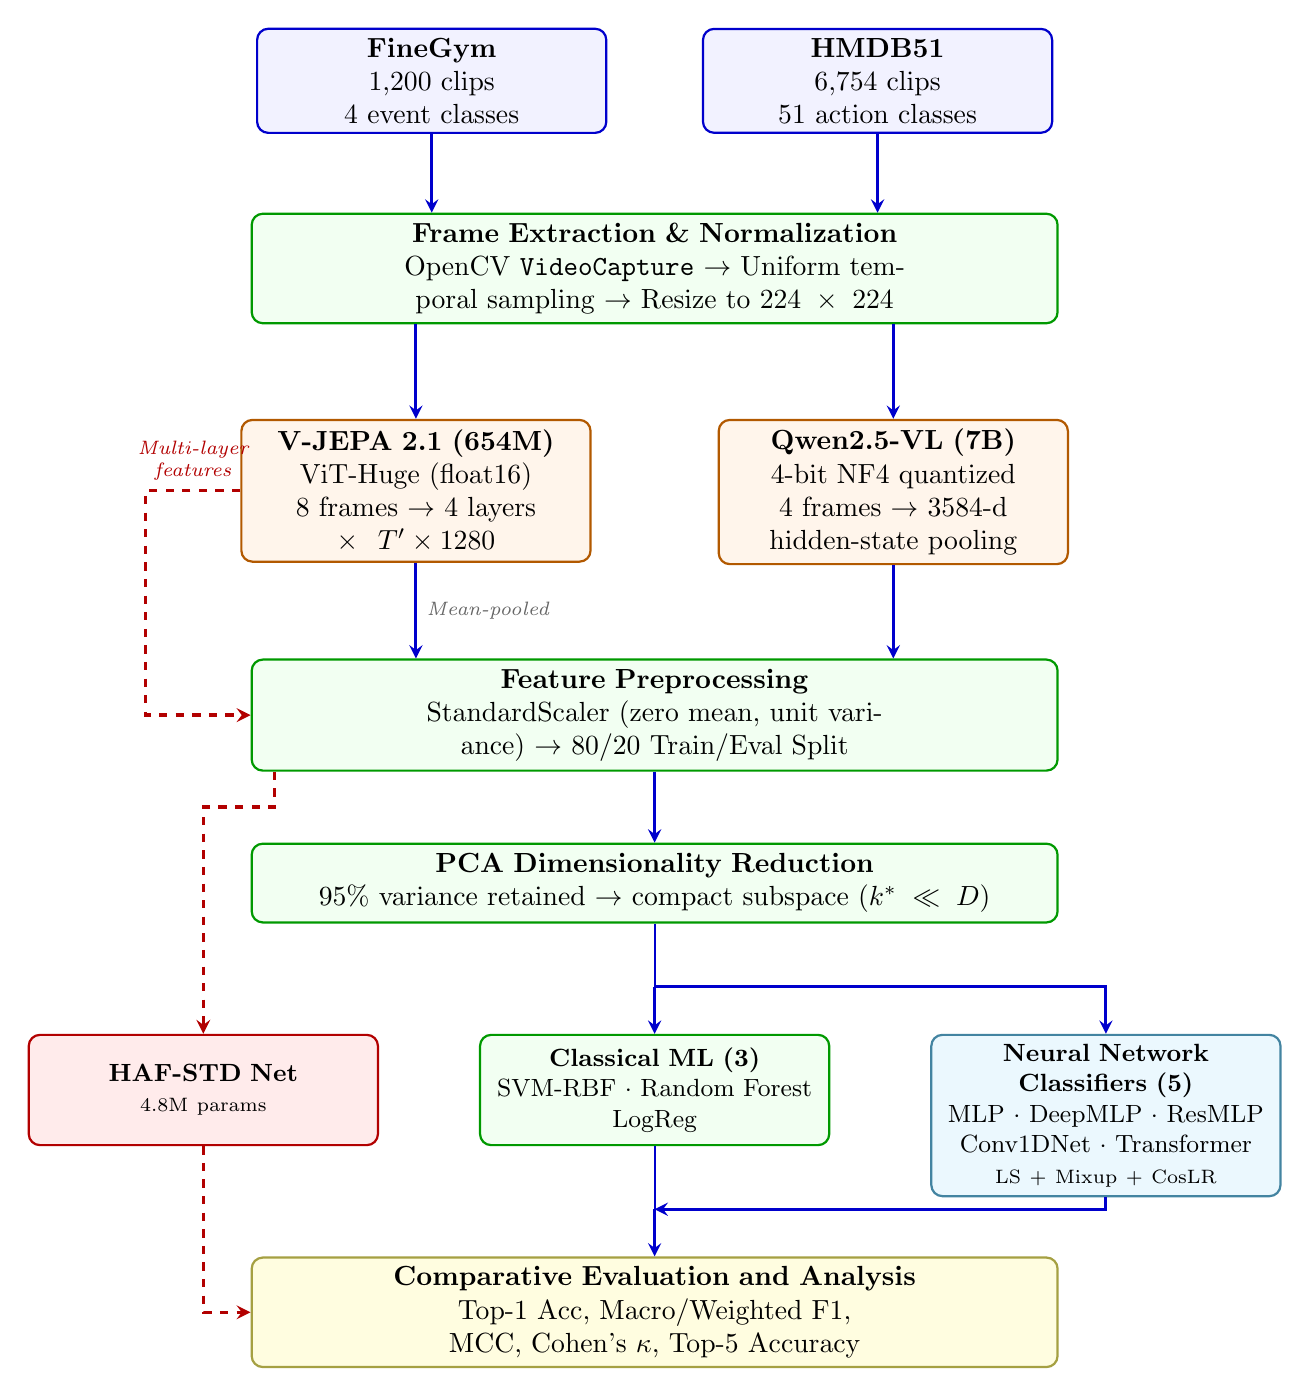
\begin{tikzpicture}[
    node distance=0.8cm,
    block/.style={rectangle, draw=blue!80!black, fill=blue!5, thick, rounded corners=4pt, text width=4.2cm, text centered, minimum height=1.0cm, font=\normalsize},
    modelblock/.style={rectangle, draw=orange!70!black, fill=orange!8, thick, rounded corners=4pt, text width=4.2cm, text centered, minimum height=1.8cm, font=\normalsize},
    procblock/.style={rectangle, draw=green!60!black, fill=green!5, thick, rounded corners=4pt, text width=10.0cm, text centered, minimum height=1.0cm, font=\normalsize},
    pcablock/.style={rectangle, draw=green!60!black, fill=green!5, thick, rounded corners=4pt, text width=10.0cm, text centered, minimum height=1.0cm, font=\normalsize},
    branchblock/.style={rectangle, draw=green!60!black, fill=green!5, thick, rounded corners=4pt, text width=4.2cm, text centered, minimum height=1.4cm, font=\small},
    trainblock/.style={rectangle, draw=cyan!60!black, fill=cyan!8, thick, rounded corners=4pt, text width=4.2cm, text centered, minimum height=1.4cm, font=\small},
    novelblock/.style={rectangle, draw=red!70!black, fill=red!8, thick, rounded corners=4pt, text width=4.2cm, text centered, minimum height=1.4cm, font=\small},
    resultblock/.style={rectangle, draw=yellow!60!black, fill=yellow!12, thick, rounded corners=4pt, text width=10.0cm, text centered, minimum height=1.0cm, font=\normalsize},
    arrow/.style={->, >=stealth, line width=1.1pt, color=blue!80!black},
    redarrow/.style={->, >=stealth, thick, line width=1.2pt, dashed, red!70!black},
]
    % === Stage 1: Data Sources ===
    \node[block] (fg_src) {\textbf{FineGym}\\1,200 clips\\4 event classes};
    \node[block, right=1.2cm of fg_src] (hmdb_src) {\textbf{HMDB51}\\6,754 clips\\51 action classes};

    % === Stage 2: Frame Extraction ===
    \node[procblock, below=1.0cm of $(fg_src.south)!0.5!(hmdb_src.south)$] (frames) {\textbf{Frame Extraction \& Normalization}\\OpenCV \texttt{VideoCapture} $\rightarrow$ Uniform temporal sampling $\rightarrow$ Resize to $224\times224$};

    % === Stage 3: Feature Extractors ===
    \node[modelblock, below left=1.2cm and 0.8cm of frames.south] (vjepa) {\textbf{V-JEPA~2.1 (654M)}\\ViT-Huge (float16)\\8 frames $\rightarrow$ 4 layers\\$\times\;T'\!\times\!1280$};
    \node[modelblock, below right=1.2cm and 0.8cm of frames.south] (qwen) {\textbf{Qwen2.5-VL (7B)}\\4-bit NF4 quantized\\4 frames $\rightarrow$ 3584-d\\hidden-state pooling};

    % === Stage 4a: Feature Preprocessing — StandardScaler (all classifiers) ===
    \node[procblock, below=1.2cm of $(vjepa.south)!0.5!(qwen.south)$] (scaler) {\textbf{Feature Preprocessing}\\StandardScaler (zero mean, unit variance) $\rightarrow$ 80/20 Train/Eval Split};

    % === Stage 4b: PCA Dimensionality Reduction (baseline classifiers only) ===
    \node[pcablock, below=0.9cm of scaler] (pca) {\textbf{PCA Dimensionality Reduction}\\95\% variance retained $\rightarrow$ compact subspace ($k^* \ll D$)};

    % === Stage 5: Classifier Branches ===
    % HAF-STD Net (far left — multi-layer features, uses StandardScaler but bypasses PCA)
    \node[novelblock, below left=1.4cm and 3.5cm of pca.south] (hafstd) {\textbf{HAF-STD Net}\\{\scriptsize 4.8M params}};
    % Classical ML (center — shared path, both models)
    \node[branchblock, below=1.4cm of pca] (classify_sk) {\textbf{Classical ML (3)}\\SVM-RBF $\cdot$ Random Forest\\LogReg};
    % Neural Network Classifiers (right — shared path, both models)
    \node[trainblock, below right=1.4cm and 3.5cm of pca.south] (classify_pt) {\textbf{Neural Network Classifiers (5)}\\MLP $\cdot$ DeepMLP $\cdot$ ResMLP\\Conv1DNet $\cdot$ Transformer\\{\scriptsize LS + Mixup + CosLR}};

    % === Stage 6: Comparative Evaluation ===
    \node[resultblock, below=1.4cm of classify_sk] (results) {\textbf{Comparative Evaluation and Analysis}\\Top-1 Acc, Macro/Weighted F1, MCC, Cohen's $\kappa$, Top-5 Accuracy};

    % ====== ARROWS ======

    % Data sources -> Frame extraction
    \draw[arrow] (fg_src.south) -- (fg_src.south |- frames.north);
    \draw[arrow] (hmdb_src.south) -- (hmdb_src.south |- frames.north);

    % Frame extraction -> Models
    \draw[arrow] (frames.south -| vjepa.north) -- (vjepa.north);
    \draw[arrow] (frames.south -| qwen.north) -- (qwen.north);

    % Models -> StandardScaler (mean-pooled features for baselines)
    \draw[arrow] (vjepa.south) -- (vjepa.south |- scaler.north)
        node[midway, right, font=\scriptsize\itshape, text=black!60] {Mean-pooled};
    \draw[arrow] (qwen.south) -- (qwen.south |- scaler.north);

    % V-JEPA multi-layer features -> StandardScaler (HAF-STD path enters preprocessing)
    \draw[redarrow] (vjepa.west) -- node[above, font=\scriptsize\itshape, text=red!70!black, align=center] {Multi-layer\\features} ++(-1.2, 0) |- (scaler.west);

    % StandardScaler -> PCA (baseline path)
    \draw[arrow] (scaler.south) -- (pca.north);

    % StandardScaler -> HAF-STD Net (bypasses PCA)
    \draw[redarrow] (scaler.south west) ++(0.3,0) -- ++(0,-.45) -| (hafstd.north);

    % PCA -> Shared classifier branches (two-way fan)
    \coordinate (fan) at ($(pca.south) + (0,-0.8)$);
    \draw[thick, color=blue!80!black] (pca.south) -- (fan);
    \draw[arrow] (fan) -- (classify_sk.north);
    \draw[arrow] (fan) -| (classify_pt.north);

    % Shared classifiers -> Comparative Evaluation (fan-in)
    \coordinate (merge) at ($(classify_sk.south) + (0,-0.8)$);
    \draw[thick, color=blue!80!black] (classify_sk.south) -- (merge);
    \draw[arrow] (merge) -- (results.north);
    \draw[arrow] (classify_pt.south) |- (merge);

    % HAF-STD -> Comparative Evaluation (dashed red path along left side)
    \draw[redarrow] (hafstd.south) |- (results.west);

\end{tikzpicture}

\caption{Flowchart depicting the proposed multi-stage experimental methodology pipeline. Solid arrows indicate the shared baseline path where mean-pooled features from both models undergo StandardScaler normalization and PCA dimensionality reduction before evaluation by 8 baseline classifiers. Dashed red arrows indicate the HAF-STD Net path, which routes V-JEPA~2.1's multi-layer temporal features through StandardScaler normalization but bypasses PCA.}
\label{fig:methodology_pipeline}
\end{figure}


\section{Data Acquisition and Dataset Characteristics}


To evaluate model performance across different task granularities, two benchmark datasets of contrasting complexity are utilized:

\subsection{FineGym Dataset (Fine-Grained Action Recognition)}
FineGym is a fine-grained activity recognition benchmark containing high-frame-rate competitive gymnastics footage. The official annotation file (v1.1) specifies precise temporal boundaries and hierarchical activity labels. In this study, evaluation focuses on the top-level Event classification tier, comprising 4 distinct gymnastics apparatus events: Balance Beam (BB), Floor Exercise (FX), Uneven Bars (UB), and Vault (VT). A balanced sample of 300 clips per class (1,200 total clips) is targeted for download via \texttt{yt-dlp} from YouTube.

\subsection{HMDB51 Dataset (General Action Recognition)}
HMDB51 is a classic benchmark for general human action recognition, curated from commercial movies and web videos. It comprises 6,754 video clips categorized into 51 action classes, encompassing facial expressions, general body motion, human-object interactions, and human-human interactions. The complete dataset is ingested directly from the Hugging Face Hub repository (\texttt{jili5044/hmdb51}).

Table~\ref{tab:dataset_comparison} summarizes the structural properties and comparative parameters of both benchmark datasets.

\begin{table}[H]
\centering
\caption{Comparison of FineGym and HMDB51 benchmark dataset specifications.}
\label{tab:dataset_comparison}
\begin{tabular}{lrr}
\toprule
\textbf{Dataset Parameter} & \textbf{FineGym (Event Level)} & \textbf{HMDB51} \\
\midrule
Task Granularity & Fine-grained (Gymnastics) & Coarse-grained (General) \\
Number of Classes & 4 & 51 \\
Target Sample Size & 1,200 clips & 6,754 clips \\
Domain Context & Uniform arena/gym environment & Diverse real-world settings \\
Primary Discriminative Cue & Subtle body kinematics & Broad motion \& background \\
Evaluation Split & 80\% Train / 20\% Test & 80\% Train / 20\% Test \\
\bottomrule
\end{tabular}
\end{table}

\section{Data Preprocessing and Input Pipeline}

Video clips undergo standardized preprocessing prior to feature extraction:
\begin{enumerate}[leftmargin=*]
    \item \textbf{Uniform Temporal Frame Sampling:} For a video clip containing $N$ total frames, a sequence of $N_f$ frames is uniformly sampled along the temporal axis:
    \begin{equation*}
        t_i = \left\lfloor i \cdot \frac{N}{N_f} \right\rfloor, \quad i \in \{0, 1, \dots, N_f - 1\}
    \end{equation*}
    For \vjepaa{}, $N_f = 8$ frames are sampled; for \qwenvl{}, $N_f = 4$ frames are sampled.
    \item \textbf{Spatial Resizing and Normalization:} Sampled frames are resized to $224 \times 224$ pixels and normalized using standard ImageNet mean ($\boldsymbol{\mu} = [0.485, 0.456, 0.406]$) and standard deviation ($\boldsymbol{\sigma} = [0.229, 0.224, 0.225]$).
\end{enumerate}

\section{Feature Extraction Framework}

Both candidate models function strictly as frozen feature extractors without updating backbone parameters.

\subsection{Self-Supervised Encoder: \vjepaa{}}
\vjepaa{} \citep{assran2025vjepa2} utilizes a ViT-Huge backbone (654M parameters) trained via non-generative spatiotemporal prediction in a latent embedding space. Given an input video sequence of 8 sampled frames, we extract two feature representations:
\begin{enumerate}[leftmargin=*]
    \item \textbf{Multi-Layer Per-Frame Features (for HAF-STD Net):} Hidden states are extracted from 4 intermediate encoder layers at 25\%, 50\%, 75\%, and 100\% depth. Spatial tokens are mean-pooled per frame, producing a tensor $\mathbf{H}_{\text{multi}} \in \mathbb{R}^{4 \times T' \times 1280}$ per clip that preserves both depth hierarchy and temporal structure.
    \item \textbf{Global Mean-Pooled Features (for Baseline Probes):} Global average pooling across all spatiotemporal tokens of the final layer outputs $\mathbf{f}_{\text{VJEPA}} \in \mathbb{R}^{1280}$.
\end{enumerate}

\subsection{V-JEPA~2.1 Self-Supervised Training Objectives}

The representational quality of the frozen \vjepaa{} encoder stems from its self-supervised pretraining objective, which performs \emph{mask-denoising prediction in representation space} rather than pixel reconstruction. Given two views $x$ and $y$ of a video, where patches have been randomly dropped from $y$, the encoder $E_\theta(\cdot)$ extracts representations from the unmasked view $x$, and a predictor $P_\phi(\cdot)$ predicts the representation of the masked view. The training objective minimizes the $\ell_1$ distance between predicted and target representations \citep{assran2025vjepa2}:
\begin{equation*}
    \underset{\theta,\,\phi,\,\Delta_y}{\text{minimize}} \quad \|P_\phi(\Delta_y, E_\theta(x)) - \operatorname{sg}(E_{\bar{\theta}}(y))\|_1
\end{equation*}
where $\Delta_y$ is a learnable mask token that indicates the locations of the dropped patches, $\operatorname{sg}(\cdot)$ denotes a stop-gradient operator to prevent representation collapse, and $\bar{\theta}$ represents an exponential moving average (EMA) of the encoder weights $\theta$. The loss is applied only to predictions of masked patches, and both the encoder $E_\theta(\cdot)$ and predictor $P_\phi(\cdot)$ are parameterized as Vision Transformers (ViTs) with Rotary Position Embedding (RoPE).

V-JEPA~2.1 \citep{murlabadia2026vjepa21} refines this objective by introducing a \emph{dense per-token prediction loss} that applies supervision individually to each masked spatiotemporal token rather than globally:
\begin{equation*}
    \mathcal{L}_{\text{predict}} = \frac{1}{|M|} \sum_{i \in M} \|P_\phi(E_\theta(x), \Delta_y)_i - \operatorname{sg}(E_{\bar{\theta}}(y)_i)\|_1
\end{equation*}
where $M$ is the set of masked patch indices from the $x$ view, and the subscript $i$ denotes the $i$-th token position. This dense formulation, combined with multi-layer intermediate supervision across encoder depth, enhances the spatial and temporal grounding of learned representations.

Figure~\ref{fig:vjepa2_arch} illustrates the complete V-JEPA~2.1 pretraining architecture. The dual-encoder framework consists of an x-Encoder $E_\theta$ that processes unmasked context tokens and a y-Encoder $E_{\bar{\theta}}$ (updated via EMA) that produces target representations. A multi-level predictor $P_\phi$ reconstructs the masked spatiotemporal token representations by fusing features across multiple encoder depths, with two complementary loss terms: a context loss ($\lambda_d \cdot L_1$) and a prediction loss ($L_1$), both applied through stop-gradient operations to prevent representational collapse.

\begin{figure}[H]
\centering
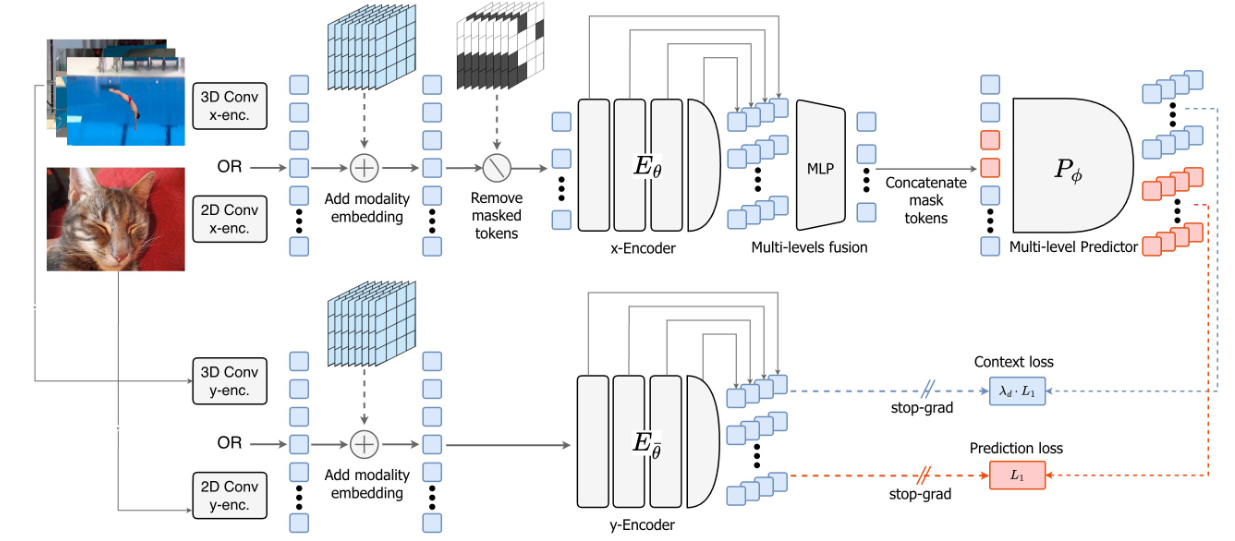
\includegraphics[width=\textwidth]{../fig/vjepa2.png}
\caption{Architecture of V-JEPA~2.1 self-supervised pretraining framework showing the dual x-Encoder and y-Encoder pipeline with multi-level fusion, mask-denoising prediction, and stop-gradient targets \citep{murlabadia2026vjepa21}.}
\label{fig:vjepa2_arch}
\end{figure}

\subsection{Vision-Language Model: \qwenvl{}}
\qwenvl{} \citep{qwen2025qwen3vl} (7B parameters) integrates a Vision Transformer encoder with a language model decoder. The model is loaded in 4-bit NormalFloat (NF4) quantization \citep{pathak2026efficientvlms}. The 4 sampled frames are passed alongside a minimal prompt (\texttt{"Describe the video action."}). The output hidden state of the final decoder layer $\mathbf{H}_{\text{decoder}} \in \mathbb{R}^{S \times 3584}$ is average-pooled across sequence tokens:
\begin{equation*}
    \mathbf{f}_{\text{Qwen}} = \frac{1}{S} \sum_{s=1}^{S} \mathbf{h}_s \in \mathbb{R}^{3584}
\end{equation*}

Figure~\ref{fig:qwen_arch} depicts the Qwen2.5-VL architecture. The model employs a Vision Encoder with a Conv3D patch embedding layer and window-partitioned attention blocks, which processes images and video frames at their native resolution. Visual tokens are then projected and interleaved with text tokens into the Qwen2.5 Language Model (LM) Decoder for autoregressive generation. Notably, the architecture uses Multimodal Rotary Position Embedding (MRoPE) with absolute time alignment for temporal grounding of video inputs and dynamic FPS sampling to accommodate variable-length video sequences.

\begin{figure}[H]
\centering
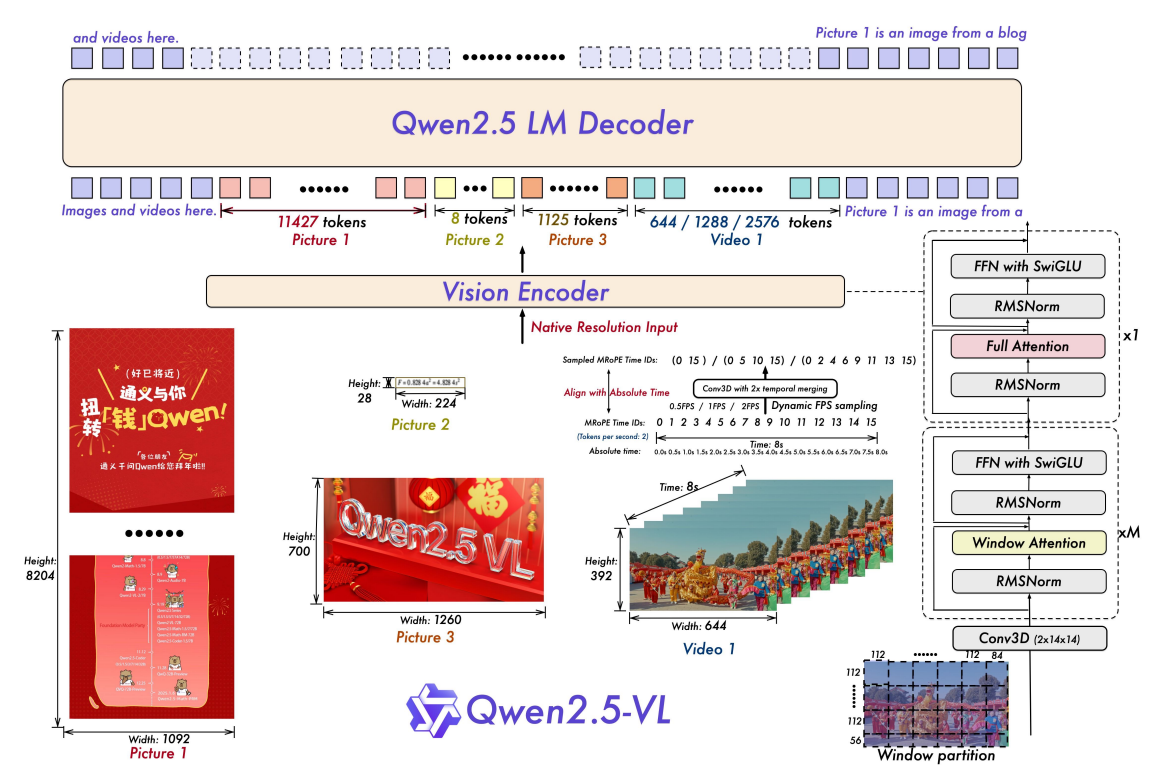
\includegraphics[width=\textwidth]{../fig/qwen.png}
\caption{Architecture of Qwen2.5-VL vision-language model illustrating the Vision Encoder with Conv3D patch embedding, window attention, and native resolution input processing, feeding into the Qwen2.5 LM Decoder with MRoPE temporal alignment \citep{qwen2025qwen3vl}.}
\label{fig:qwen_arch}
\end{figure}

\section{Feature Standardization and Dimensionality Reduction}

To ensure optimal classifier convergence and mitigate the curse of dimensionality, extracted feature vectors undergo standard transformations:
\begin{enumerate}[leftmargin=*]
    \item \textbf{Z-Score Standardization:} Feature vectors $\mathbf{x}_i$ are standardized using training set statistics:
    \begin{equation*}
        \mathbf{z}_i = \frac{\mathbf{x}_i - \boldsymbol{\mu}_{\text{train}}}{\boldsymbol{\sigma}_{\text{train}}}
    \end{equation*}
    \item \textbf{Principal Component Analysis (PCA):} PCA is fitted on the standardized training feature matrix $\mathbf{Z}_{\text{train}}$ to project representations onto an orthogonal subspace while retaining 95\% of total variance:
    \begin{equation*}
        K = \arg\min_k \left\{ \frac{\sum_{j=1}^k \lambda_j}{\sum_{m=1}^D \lambda_m} \ge 0.95 \right\}
    \end{equation*}
\end{enumerate}

\section{Downstream Baseline Classifiers}

An ensemble of 8 baseline classifiers (3 classical ML and 5 neural network classifiers) is evaluated on the transformed feature representations:

\subsection{Classical Machine Learning Classifiers}
\begin{enumerate}[leftmargin=*]
    \item \textbf{Support Vector Machine (SVM-RBF):} RBF kernel with $C=10.0$ and balanced class weighting.
    \item \textbf{Random Forest:} Ensemble of 500 decision trees with Gini impurity split criteria.
    \item \textbf{Softmax Logistic Regression:} Multinomial linear probe with L2 regularization ($C=1.0$).
\end{enumerate}

\subsection{Neural Network Classifier Architectures}
\begin{enumerate}[leftmargin=*]
    \item \textbf{Multi-Layer Perceptron (MLP):} Scikit-learn MLP with two hidden layers (512, 256) and adaptive learning rate.
    \item \textbf{DeepMLP:} 4-layer feedforward network (512 $\rightarrow$ 256 $\rightarrow$ 128 $\rightarrow$ Classes) with BatchNorm, GELU, and Dropout (0.3).
    \item \textbf{ResMLP:} Deep residual MLP with 3 residual blocks: $\mathbf{h}_{l+1} = \text{GELU}(\mathbf{h}_l + \mathcal{F}(\mathbf{h}_l))$.
    \item \textbf{Conv1DNet:} 1D CNN treating feature dimensions as sequence channels.
    \item \textbf{MiniTransformer:} 2-layer Transformer Encoder with multi-head self-attention ($h=4$) on chunked feature embeddings.
\end{enumerate}

All neural network baseline models are trained using label smoothing ($\epsilon=0.1$), feature-space mixup ($\alpha=0.2$), Cosine Annealing LR scheduling, and early stopping.

\section{Proposed Classifier Architecture: HAF-STD Net}
\label{sec:proposal_hafstd}

As a key technical contribution of this thesis, we propose HAF-STD Net (Hierarchical Adaptive Fusion with Spectral-Temporal Decomposition), a classification architecture (4.8M parameters) specifically tailored for frozen V-JEPA~2.1 backbones. HAF-STD Net operates on multi-layer per-frame features $\mathbf{H} \in \mathbb{R}^{4 \times T' \times 1280}$ and incorporates three core mechanisms:

\subsection{1. Spectral-Temporal Decomposition via 1D Haar DWT}
At each selected layer $k \in \{1, 2, 3, 4\}$, a 1D Haar Discrete Wavelet Transform is applied along the temporal dimension $T'$:
\begin{equation*}
    \mathbf{a}_k = \frac{1}{2}(\mathbf{h}_{2t} + \mathbf{h}_{2t+1}), \quad
    \mathbf{d}_k = \frac{1}{2}(\mathbf{h}_{2t} - \mathbf{h}_{2t+1})
\end{equation*}
where $\mathbf{a}_k$ isolates low-frequency static appearance features and $\mathbf{d}_k$ isolates high-frequency motion dynamics.

\subsection{2. Inter-Layer Representation Velocity}
Inter-layer deltas are computed between consecutive encoder layers to quantify representation velocity across depth:
\begin{equation*}
    \Delta\mathbf{H}_k = \bar{\mathbf{H}}_{k+1} - \bar{\mathbf{H}}_k
\end{equation*}
where $\bar{\mathbf{H}}_k$ is the temporally mean-pooled representation at layer $k$.

\subsection{3. Adaptive Routing and Cosine Classification}
The 3 streams per layer (appearance, motion, velocity) yield $4 \times 3 = 12$ projected feature streams $\mathbf{s}_i \in \mathbb{R}^{256}$. An adaptive routing network computes input-dependent softmax weights $\mathbf{w} \in \mathbb{R}^{12}$:
\begin{equation*}
    \mathbf{w} = \text{softmax}\left(\text{MLP}\left([\mathbf{s}_1; \mathbf{s}_2; \dots; \mathbf{s}_{12}]\right)\right), \quad
    \mathbf{f} = \sum_{i=1}^{12} w_i \cdot \mathbf{s}_i
\end{equation*}
The dynamically fused feature $\mathbf{f}$ is classified via a cosine-similarity head with temperature scaling $\tau$:
\begin{equation*}
    P(y = c \mid \mathbf{f}) = \frac{\exp\left(\tau \cdot \hat{\mathbf{f}}^T \hat{\mathbf{w}}_c\right)}{\sum_{j=1}^C \exp\left(\tau \cdot \hat{\mathbf{f}}^T \hat{\mathbf{w}}_j\right)}
\end{equation*}

\section{Performance Evaluation Metrics}

Model performance across both datasets is evaluated using standard metrics:
\begin{itemize}[leftmargin=*]
    \item \textbf{Macro F1-Score:} Unweighted mean of class F1-scores.
    \item \textbf{Matthews Correlation Coefficient (MCC):} Balanced metric robust to class imbalance.
    \item \textbf{Cohen's Kappa ($\kappa$):} Chance-corrected classification agreement.
\end{itemize}

Experiments are conducted on Kaggle cloud platform using NVIDIA Tesla T4 GPUs (16 GB VRAM) with PyTorch 2.1, Hugging Face Transformers, and Scikit-Learn.

% =============================================================================
%    CHAPTER 4: WORK PLAN AND EXPECTED OUTCOMES
% =============================================================================
\chapter{Work Plan and Expected Outcomes}

\section{Work Plan of the Study}

The proposed research will be conducted over a 14-week timeline. Figure~\ref{fig:gantt_chart} illustrates the Gantt chart detailing the proposed project phases and execution timeline.

\begin{figure}[H]
\centering
\resizebox{\textwidth}{!}{%
\begin{ganttchart}[
    hgrid,
    vgrid,
    x unit=0.55cm,
    y unit title=0.6cm,
    y unit chart=0.6cm,
    title height=1,
    bar/.style={fill=blue!40},
    bar label font=\small,
    title label font=\small,
    milestone label font=\small,
    group label font=\small\bfseries,
]{1}{14}
    \gantttitle{Weeks}{14} \\
    \gantttitlelist{1,...,14}{1} \\

    \ganttbar{Literature Survey \& Analysis}{1}{3} \\
    \ganttbar{Proposal Preparation \& Defense}{3}{4} \\
    \ganttbar{Dataset Ingestion \& Sampling}{5}{6} \\
    \ganttbar{Feature Extraction (V-JEPA 2 \& Qwen2.5-VL)}{6}{8} \\
    \ganttbar{Classifier Probing \& HAF-STD Net}{8}{10} \\
    \ganttbar{Comparative Analysis \& Validation}{10}{11} \\
    \ganttbar{Thesis Documentation \& Drafting}{11}{13} \\
    \ganttbar{Final Review \& Defense Submission}{13}{14}
\end{ganttchart}%
}
\caption{Gantt Chart illustrating the 14-week proposed research timeline.}
\label{fig:gantt_chart}
\end{figure}

Table~\ref{tab:schedule} details the core activities and milestones planned for each phase of the research.

\begin{table}[H]
\centering
\caption{Detailed timeline breakdown and major project milestones.}
\label{tab:schedule}
\begin{tabular}{llp{7.5cm}}
\toprule
\textbf{Phase} & \textbf{Timeline} & \textbf{Description of Activities} \\
\midrule
Literature Survey & Weeks 1--3 & Comprehensive literature review of SSL video encoders, VLMs, fine-grained activity benchmarks, and gap analysis. \\
Proposal Defense & Weeks 3--4 & Preparation, submission, and defense of the Master's thesis proposal document. \\
Data Acquisition & Weeks 5--6 & Automated ingestion of FineGym clips via \texttt{yt-dlp} and extraction of HMDB51 dataset from Hugging Face Hub. \\
Feature Extraction & Weeks 6--8 & Batch extraction of multi-layer and global features from \vjepaa{} and \qwenvl{} on Kaggle Tesla T4 GPU. \\
Classifier & Weeks 8--10 & Feature standardization, PCA fitting, training 8 baseline classifiers (3 classical ML + 5 neural network classifiers) and developing the \textbf{HAF-STD Net} architecture. \\
Statistical Analysis & Weeks 10--11 & Cross-granularity performance comparison, HAF-STD Net vs baseline probe ablation, error matrix evaluation. \\
Documentation & Weeks 11--13 & Comprehensive drafting of Master's thesis chapters, figures, tables, and appendices. \\
Thesis Submission & Weeks 13--14 & Plagiarism verification, peer review, supervisor approval, and final thesis defense submission. \\
\bottomrule
\end{tabular}
\end{table}

\section{Expected Outcomes}

The primary expected outcomes of this research project include:
\begin{enumerate}[leftmargin=*]
    \item \textbf{Empirical Feature Quality Evaluation:} Quantitative performance benchmarks comparing frozen representations from self-supervised video encoders (\vjepaa{}, 654M) against vision-language models (\qwenvl{}, 7B).
    \item \textbf{Proposed Classifier Contribution (HAF-STD Net):} A classification architecture (4.8M parameters) combining 1D Haar wavelet spectral-temporal decomposition, depth representation velocity, and adaptive routing for frozen self-supervised backbones.
    \item \textbf{Granularity-Dependent Representation Insights:} Detailed comparative evidence demonstrating how self-supervised latent prediction vs.\ multimodal language pre-training performs across fine-grained (FineGym) vs.\ coarse-grained (HMDB51) action classification.
    \item \textbf{Parameter Efficiency Analysis:} Practical guidelines establishing whether compact, video-specialized encoders can outperform general-purpose 7B vision-language models on specialized motion tasks.
    \item \textbf{Classifier Compatibility Assessment:} Identification of optimal classical machine learning models and neural network classifiers (ResMLP, DeepMLP, HAF-STD Net) for downstream representation spaces.
    \item \textbf{Publication Artifacts:} A complete Master's thesis report, open-source experimental codebase, and clean dataset feature benchmarks for future research.
\end{enumerate}



% --- Back Matter -------------------------------------------------------------
\clearpage
% --- References (APA 7th Edition via biblatex-apa) ---
\printbibliography[title={References}]
\addcontentsline{toc}{chapter}{References}

\end{document}

